%%%%%%%%%%%%%%%%%%%%%%%%%%%%%%%%%%%%%%%%%
% Short Sectioned Assignment
% LaTeX Template
% Version 1.0 (5/5/12)
%
% This template has been downloaded from:
% http://www.LaTeXTemplates.com
%
% Original author:
% Frits Wenneker (http://www.howtotex.com)
%
% License:
% CC BY-NC-SA 3.0 (http://creativecommons.org/licenses/by-nc-sa/3.0/)
%
%%%%%%%%%%%%%%%%%%%%%%%%%%%%%%%%%%%%%%%%%

%----------------------------------------------------------------------------------------
%	PACKAGES AND OTHER DOCUMENT CONFIGURATIONS
%----------------------------------------------------------------------------------------

\documentclass[paper=a4, fontsize=11pt]{scrartcl} % A4 paper and 11pt font size

\usepackage[T1]{fontenc} % Use 8-bit encoding that has 256 glyphs
%\usepackage{fourier} % Use the Adobe Utopia font for the document - comment this line to return to the LaTeX default
\usepackage[english]{babel} % English language/hyphenation
\usepackage{amsmath,amsfonts,amsthm} % Math packages

\usepackage{lipsum} % Used for inserting dummy 'Lorem ipsum' text into the template

\usepackage{graphicx}
\usepackage{caption}
\usepackage{subcaption}

\usepackage{sectsty} % Allows customizing section commands
\allsectionsfont{\centering \normalfont\scshape} % Make all sections centered, the default font and small caps

\usepackage{fancyhdr} % Custom headers and footers
\pagestyle{fancyplain} % Makes all pages in the document conform to the custom headers and footers
\fancyhead{} % No page header - if you want one, create it in the same way as the footers below
\fancyfoot[L]{} % Empty left footer
\fancyfoot[C]{} % Empty center footer
\fancyfoot[R]{\thepage} % Page numbering for right footer
\renewcommand{\headrulewidth}{0pt} % Remove header underlines
\renewcommand{\footrulewidth}{0pt} % Remove footer underlines
\setlength{\headheight}{13.6pt} % Customize the height of the header

\numberwithin{equation}{section} % Number equations within sections (i.e. 1.1, 1.2, 2.1, 2.2 instead of 1, 2, 3, 4)
\numberwithin{figure}{section} % Number figures within sections (i.e. 1.1, 1.2, 2.1, 2.2 instead of 1, 2, 3, 4)
\numberwithin{table}{section} % Number tables within sections (i.e. 1.1, 1.2, 2.1, 2.2 instead of 1, 2, 3, 4)

\setlength\parindent{0pt} % Removes all indentation from paragraphs - comment this line for an assignment with lots of text

%----------------------------------------------------------------------------------------
%	TITLE SECTION
%----------------------------------------------------------------------------------------

\newcommand{\horrule}[1]{\rule{\linewidth}{#1}} % Create horizontal rule command with 1 argument of height

\title{	
\normalfont \normalsize 
\textsc{ETH Zurich, D-INFK} \\ [25pt] % Your university, school and/or department name(s)
\horrule{0.5pt} \\[0.4cm] % Thin top horizontal rule
\huge Computer Vision Exercise 10 \\ % The assignment title
\horrule{2pt} \\[0.5cm] % Thick bottom horizontal rule
}

\author{Igor Pesic} % Your name

\date{\normalsize\today} % Today's date or a custom date

\begin{document}

\maketitle % Print the title


\section{Image Categorization}

\subsection{Pipeline}

I have implemented the pipeline as it was described in the exercise sheet. The main steps are as following:
\begin{itemize}
\item Extract the points on the mesh gird from the image
\item Calculate the descriptor for each point on the grid. Descriptor is the histogram of oriented gradients. These are also called "visual words."
\item Constructing of the codebook: cluster all the descriptors from the class-1 images with k-means and choose the centroids to be representative "words" in the vocabulary.
\item Represent each word with the bag of words from the vocabulary. Here I build the histogram of words for each image.
\item Classify the test images based on the "bag-of-words" representation. Here I have implemented both nearest neighbor and Bayesian classifier.
\end{itemize}

\subsection{Choosing K}

Here I am going to shortly present my choice of K for the k-means. In Figure \ref{fig:diff_k} I have plotted the loss (sum of distances from each data point to its cluster center) for different K-s. X-Axis represent different K-s and Y-Axis are the losses. As expected, the loss decreases for higher K, but there is no clear K for which we can notice the biggest impact. I have run the k-means 10 times for each value of K to get more accurate results.\\

\begin{figure}
\centering
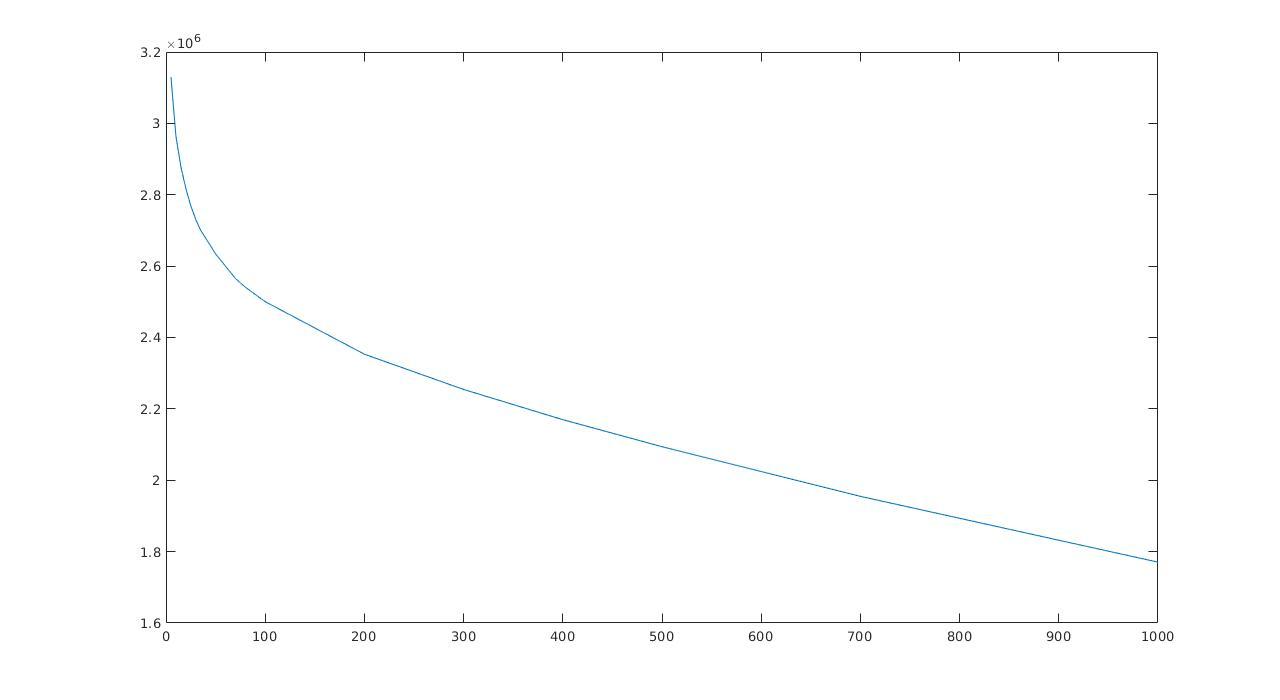
\includegraphics[width=0.9\textwidth]{loss_with_k.jpg}
\caption{Loss for different K.}
\label{fig:diff_k}
\end{figure}

Also I have compared the classification results for $K = [70, 150, 300]$ and I have noticed the improvement of Bayesian classifier with lower K and pretty random results with NN classifier. Thus I have decided to choose $K=70$.

\subsection{Nearest Neighbor vs Bayesian Classifier}

As mentioned above, the results obtained by Bayesian classifier were more stable then those of NN classifier which is to be expected since NN with only 1 neighbor is very sensitive to outliers. The Table \ref{tab:res} represents the results obtained by running the algorithm 3 times for each configuration.

\begin{table}
\begin{center}
    \begin{tabular}{| l | l | l | l |}
    \hline
    K & 70 & 150 & 300 \\ \hline
    NN & 0.87, 0.9, 0.92 & 0.79, 0.83, 0.99 & 0.82, 0.91, 0.93 \\ \hline
    Bayesian & 0.85, 0.86, 0.9 & 0.73, 0.78, 0.78 & 0.7, 0.72, 0.77 \\ \hline
    \end{tabular}
    \caption{Results for different classifiers and different K. Each cell contains classification accuracy obtained in 3 trials.}
    \label{tab:res}
\end{center}
\end{table}
 
As we can see from the table, the NN classifier seems to have better performance on average.

\end{document}